\documentclass{standalone}
\usepackage{tikz}
\usetikzlibrary{shapes.geometric, positioning}

\begin{document}

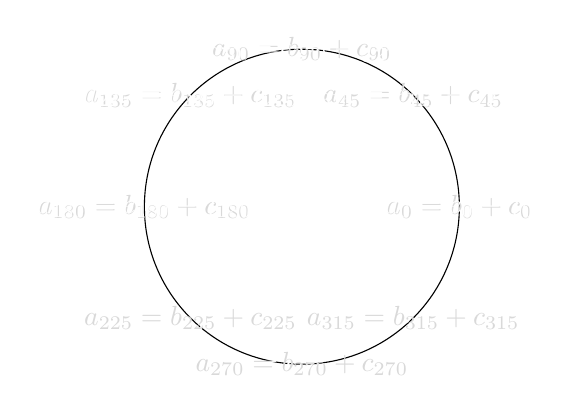
\begin{tikzpicture}[scale=2]
    % Define colors
    \colorlet{gray1}{gray!30}
    \colorlet{white1}{white}
    
    % Draw the circle
    \draw (0,0) circle (1);
    
    % Define angles for each part
    \foreach \i in {0,45,90,135,180,225,270,315} {
        % Calculate the coordinates for each point
        \pgfmathsetmacro{\x}{cos(\i)}
        \pgfmathsetmacro{\y}{sin(\i)}
        
        % Place the first equation in each part
        \node[align=center] at (\x,\y) {\textcolor{gray1}{$a_{\i} = b_{\i} + c_{\i}$}};
        
        % Place the second equation in each part
        \node[align=center] at (\x,-\y) {\textcolor{white1}{$d_{\i} = e_{\i} - f_{\i}$}};
    }
\end{tikzpicture}

\end{document}